\documentclass[tikz,border=8pt]{standalone}
\usetikzlibrary{arrows.meta,positioning}
\begin{document}
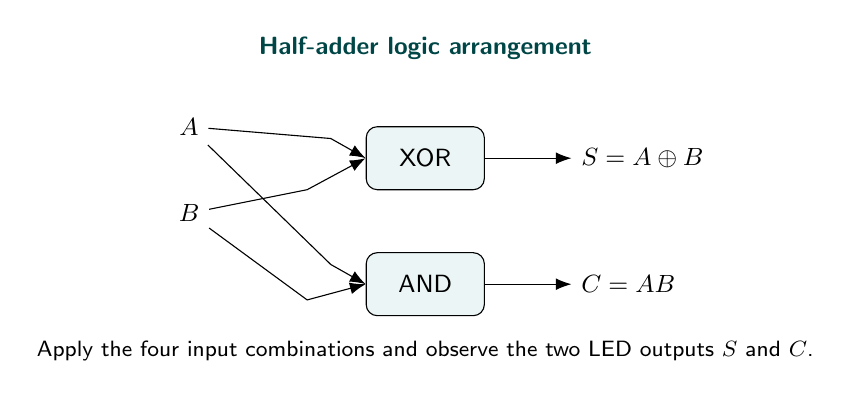
\begin{tikzpicture}[font=\sffamily\small]
\node[font=\sffamily\bfseries\small,text=teal!55!black] at (0,3.4) {Half-adder logic arrangement};
\node[draw,rounded corners,fill=teal!8,minimum width=1.5cm,minimum height=.8cm] (xor) at (0,2) {XOR};
\node[draw,rounded corners,fill=teal!8,minimum width=1.5cm,minimum height=.8cm] (and) at (0,.4) {AND};
\node (a) at (-3,2.4) {$A$}; \node (b) at (-3,1.3) {$B$};
\draw[-{Latex[length=2mm]}] (a)--(-1.2,2.25)--(xor.west); \draw[-{Latex[length=2mm]}] (a)--(-1.2,.65)--(and.west);
\draw[-{Latex[length=2mm]}] (b)--(-1.5,1.6)--(xor.west); \draw[-{Latex[length=2mm]}] (b)--(-1.5,.2)--(and.west);
\node[right=1.1cm of xor] (sum) {$S=A\oplus B$};
\node[right=1.1cm of and] (carry) {$C=A B$};
\draw[-{Latex[length=2mm]}] (xor.east)--(sum); \draw[-{Latex[length=2mm]}] (and.east)--(carry);
\node[font=\sffamily\footnotesize] at (0,-.45) {Apply the four input combinations and observe the two LED outputs $S$ and $C$.};
\end{tikzpicture}
\end{document}
